\chapter{Multi-robot Smoothing and Mapping}
\label{chap:two}

%In this chapter, I will introduce several key basic concepts and the associated terminologies of factor graph \cite{factorgraph} along with its SLAM formulation as proposed by Dellart and Kaess [ref] but for the scenario of multiple robots. A factor graph is a type of probabilistic graphical model which represents the factorization of a probabilistic distribution function. They are used to model complex estimation problems having wide range of applications in robotics. Formulating the SLAM problem using the factor graph, also known as pose graph in the robotics literature, opens the door for the application of several probabilistic inference algorithms. Our research is multi-robot SLAM and we will use this as an example throughout the paper. Also, the solution to the SLAM problem using the recent pose graph representations has garnered much attention because of their computational efficiency and robustness. 

In this chapter, I will review the SLAM formulation using probabilistic inference as proposed by Dellaert and Kaess \cite{dellaertsam} but for the scenario of multiple robots. It is referred as the \textit{full} SLAM problem as it contains the entire trajectory and all the landmarks in the state vector. The solution to the SLAM problem using the recent pose graph representations has garnered much attention because of their computational efficiency and robustness. In our work, we will be using the Incremental Smoothing and Mapping using the Bayes tree (ISAM2) \cite{kaessisam2} as the optimization algorithm for SLAM. Improvements on efficiency of variable reordering for combined graphs, support for cooperative mapping and multi-robot relative pose initialization are demonstrated as an extension to ISAM2. I will also introduce a few key concepts and terminologies of factor graph \cite{factorgraph} aiding in the better understanding of the contributions in this thesis. A factor graph is a type of probabilistic graphical model which represents the factorization of a probabilistic distribution function. They are used to model complex estimation problems having wide range of applications in robotics. Formulating the SLAM problem using the factor graph, also known as pose graph in the robotics literature, opens the door for the application of several probabilistic inference algorithms. Although the proposed variable reordering is applicable to any general sparse linear system, our research is multi-robot SLAM and we will use this as an example for formulation throughout the paper. However, to demonstrate its capability outside SLAM, we present some results on the real-world datasets from SuiteSparse \cite{suitesparse} in Chapter \ref{chap:three}.
\paragraph{}
In the following section, I will describe the graph structure underlying the multi-robot SLAM which leads to the optimization problem. I then briefly explain the various factorization schemes available upon linearization. I continue with providing an insight on how the various components of the graph are linked with their equivalent matrix representations. The chapter concludes by providing sufficient motivation and getting into the crux of the contribution i.e. efficient variable reordering for fused factor graphs. 

\section{Cooperative SLAM as Probabilistic Inference}
In the case of SLAM, the set of constraints obtained from the proprioceptive sensors like odometry measurements, inertial measurement units (IMUs) and exteroceptive sensors like range (LIDAR) and vision measurements form a Markov chain that connects all the variables to be estimated. Consider a single robot navigation task whose pose variables are given by $X = \{\textbf{x}_i\}_{i=0}^{i=N}$, input commands by $U = \{\textbf{u}_i\}_{i=1}^{i=N}$, sensor observations by $Z = \{\textbf{z}_k\}_{k=0}^{i=M}$ and the landmarks as $L = \{\textbf{l}_j\}_{j=1}^{j=K}$. The belief network showing the interrelationship between these variables is given in Figure \ref{fig:single_bel_net}. The estimation of these variables is given by the following probabilistic formulation: 
\begin{equation}
P(X,U,Z,L) = p(\textbf{x}_0)\prod_{i=1}^{N}p(\textbf{x}_i\mid \textbf{x}_{i-1}, \textbf{u}_i) \prod_{k=0}^{M}p(\textbf{z}_k\mid \textbf{x}_{i_k}, \textbf{l}_{j_k})
\label{eq:jp}
\end{equation}
where $p(\textbf{x}_0)$ is the prior over the initial pose of the robot, $p(\textbf{x}_i\mid \textbf{x}_{i-1}, \textbf{u}_i)$ represents the process model or the motion model that gives the next pose $x_i$ based on the control input $\textbf{u}_i$ and $p(\textbf{z}_k\mid \textbf{x}_{i_k}, \textbf{l}_{j_k})$ represents the measurement model. The measurement model is parametrized by the current pose $\textbf{x}_i$ that is obtained from the motion model. Throughout this explanation, I assume known correspondence between the landmark and measurement $(i_k, j_k)$. However, in our experiments this correspondence is obtained from data association as described in Chapter \ref{chap:five}. 
%\input{Chapters/figures2/single_robot_belief_network}
\begin{figure}
\centering
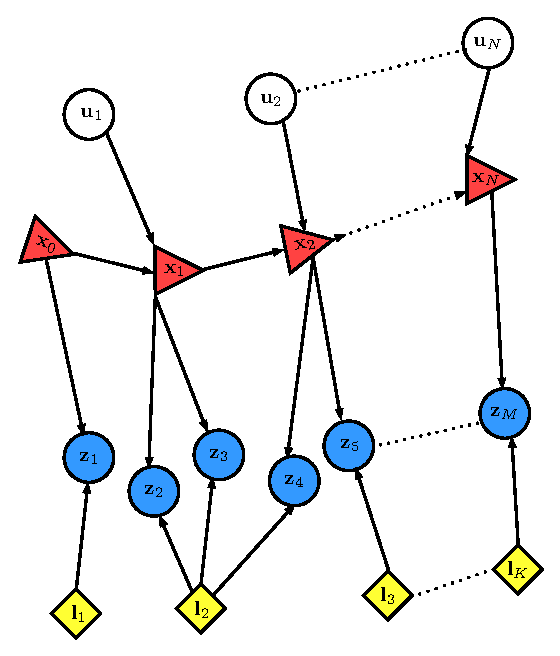
\includegraphics{Chapters/figures2/single_robot_belief_network}
\caption{The belief network showing the cause-effect relationship of a robot navigation scenario. The robot (red) is given action inputs (plain) to navigate and collect landmark (yellow) measurements (blue). Same landmarks detected at multiple observations from a single pose indicates duplication which will be solved by data association.}
\label{fig:single_bel_net}
\end{figure}
\paragraph{}
I consider Gaussian noise in the process and measurement models following the standard assumption in SLAM literature \cite{thrunprobabilistic}. The below formulation differs slightly from the typical way it is done in the SLAM papers as needed for our implementation and walking through it would provide a clear picture. The process model relating the previous pose $\textbf{x}_{i-1}$ and the control input $\textbf{u}_i$ with the ground truth value of current pose $\textbf{x}_i$ is: 
\begin{equation}
\textbf{x}_i = f(\textbf{x}_{i-1},\textbf{u}_i) + \textbf{w}_p
\label{eq:procmod}
\end{equation}
where $f(.)$ is the odometry model and $\textbf{w}_p$ is the normally distributed zero mean process noise with variance $\Lambda$. The previous pose $\textbf{x}_{i-1}$ is obtained from recursion and a prior over the very first pose is provided as a starting point. The equation can be understood as expressing the gap between the model and the ground truth with noise $\textbf{w}_p \sim \mathcal{N}(0,\Lambda)$. Since this noise parameter only captures the local variation between two poses it is a valid approximation owing to data coming from sensors at a high frequency. We also use point-to-line metric based Iterative Closest Point (ICP) \cite{csmicp} for laser scan-matching which is another source for obtaining local transform measurement between every successive pose of the robot. The laser scan matching model is given by:
\begin{equation}
\textbf{x}_i = \textbf{x}_{i-1} + s(\textbf{d}_{i-1}, \textbf{d}_i) + \textbf{w}_s
\label{eq:scanmod}
\end{equation}
where $s(.)$ is the laser scan-matching model, $\textbf{d}_{i-1}$ and $\textbf{d}_{i}$ are the scan ranges obtained at $\textbf{x}_{i-1}$ and $f(\textbf{x}_{i-1}, \textbf{u}_i)$ respectively and $\textbf{w}_s$ is the normally distributed zero mean process noise with variance $\Omega$. A curious reader can refer Appendix 2 [update] for a better description of motion and scan-matching models. The measurement model relating the current pose obtained from the process model, the landmark pose $\textbf{l}_j$ and the ground truth landmark pose $\textbf{z}_k$ is:
\begin{equation}
\textbf{z}_k = h(f(\textbf{x}_{i-1}, \textbf{u}_i) + \textbf{w}_p, \textbf{l}_k) + \textbf{w}_m
\label{eq:measmod}
\end{equation}
where $h(.)$ is the measurement model, $\textbf{w}_m$ is the zero mean Gaussian measurement noise with variance $\Gamma$. Using the above Equations \ref{eq:procmod}, \ref{eq:scanmod} and \ref{eq:measmod} to express the probability distributions in Equation \ref{eq:jp}:
\begin{equation}
p(\textbf{x}_i \mid \textbf{x}_{i-1}, \textbf{u}_i)  \propto \text{exp} \biggl(-\frac{1}{2} \biggl( \frac{1}{8}\norm{\textbf{x}_{i-1} + s(\textbf{d}_{i-1}, \textbf{d}_i) - f(\textbf{x}_{i-1},\textbf{u}_i)}_{\Xi}^2 + \frac{1}{2} \text{ln} \frac{\mid \Xi \mid}{\sqrt{\mid \Lambda \mid \mid \Omega \mid}}\biggr)\biggr)
\label{eq:procdist}
\end{equation}
where
$$\Xi = \frac{\Lambda+\Omega}{2}$$
\begin{equation}
p(\textbf{z}_k\mid \textbf{x}_{i_k}, \textbf{l}_{j_k}) \propto \text{exp} \biggl(-\frac{1}{2} \biggl( \frac{1}{8}\norm{\textbf{z}_{k} - h(f(\textbf{x}_{i-1}, \textbf{u}_i) + \textbf{w}_p, \textbf{l}_j)}_{\Psi}^2 + \frac{1}{2} \text{ln} \frac{\mid \Psi \mid}{\sqrt{\mid \Lambda \mid \mid \Gamma \mid}}\biggr)\biggr)
\label{eq:measdist}
\end{equation}
where
$$\Psi = \frac{\Lambda+\Gamma}{2} $$
The distance measure raised by the exponential term in the above equations are given by the Bhattacharyya distance \cite{Bhattacharyya} between the noise distributions of different sensor models. It is more reliable than the usual Mahalanobis distance formulation for finding the distance between distributions of different standard deviations. 

\textbf{Remark:} We denoted $\textbf{x}_{i}$ as the ground truth value of the current pose. However, in practise ground truth is either not available or extremely difficult to obtain. But it has to be noted that none of the above equations in this section has $\textbf{x}_i$ term on the right hand side. This means that we do not require the ground truth for any of our calculations and only require the previous pose $\textbf{x}_{i-1}$ which is obtained by forward simulating the process model during the last iteration. Effectively, all that is represented by the Equation \ref{eq:procdist} and \ref{eq:measdist} are the distributions of error between various sensor models.

\subsection{Formulating as Optimization}
The optimal estimate of the unknown variables is obtained by minimizing the error distribution. The error distribution that is obtained in the previous subsection eventually becomes the cost function to be optimized. The error magnitude given by $\norm{.}^2$ in Equation \ref{eq:procdist} and \ref{eq:measdist} has to be minimum for the probabilities to attain maximum. Note that the constant natural logarithm term is immaterial in the optimization. This is called as Maximum a Posteriori (MAP) estimate of the unknown variables. The problem could easily be converted in to non-linear least squares optimization to take advantage of the state-of-the-art sparse solvers based on Gauss-Newton or the Levenberg-Marquardt algorithm \cite{lsopt}. The estimate of the unknown variables at peak probability from Equation \ref{eq:jp}:
\begin{equation}
\Theta^* = \text{arg} \max_{\Theta} P(X,U,Z,L)
\end{equation}
where $\Theta = [X;L]$ and $\Theta^* = [X^*;L^*]$ is the augmented state vector containing all the state and landmark unknowns. Maximizing the above function is equal to minimizing its negative log likelihood:
\begin{equation}
\Theta^* = \text{arg} \min_{\Theta} -\text{ln} \ P(X,U,Z,L)
\end{equation}
This gives the most famous non-linear Least Squares formulation of the SLAM problem:
\begin{multline}
\Theta^* = \text{arg} \min_{\Theta} \biggl\{ \frac{N}{16} \sum_{i=1}^{N} \norm{\textbf{x}_{i-1} + s(\textbf{d}_{i-1}, \textbf{d}_i) - f(\textbf{x}_{i-1},\textbf{u}_i)}_{\Xi}^2 + \\ \frac{M}{16} \sum_{k=1}^{M} \norm{\textbf{z}_{k} - h(f(\textbf{x}_{i-1}, \textbf{u}_i) + \textbf{w}_p, \textbf{l}_j)}_{\Psi}^2 + \frac{1}{4} \text{ln} \biggl( \frac{\mid \Xi \mid \mid \Psi \mid}{\mid \Lambda \mid \sqrt{\mid \Omega \mid \mid \Gamma \mid}} \biggr) \biggr\}
\label{eq:lsopt}
\end{multline}
where $\norm{\textbf{e}}_\Sigma = \textbf{e}^{\top}\Sigma^{-1}\textbf{e}$. Although the constant natural logarithm term does not matter during optimization it is necessary to include it in case of time varying covariance as used by us. 

\subsection{Optimization for Multiple robots}
Formulating the optimization objective for multiple robots is simple once the Equation \ref{eq:lsopt} is given. However, the difficulty arises during real-time implementation as it involves online fusing of multiple factor graphs and initializing the relative pose graphs. The next two chapters exclusively contributes towards that by introducing smart numerical techniques. 
\begin{figure}
\centering
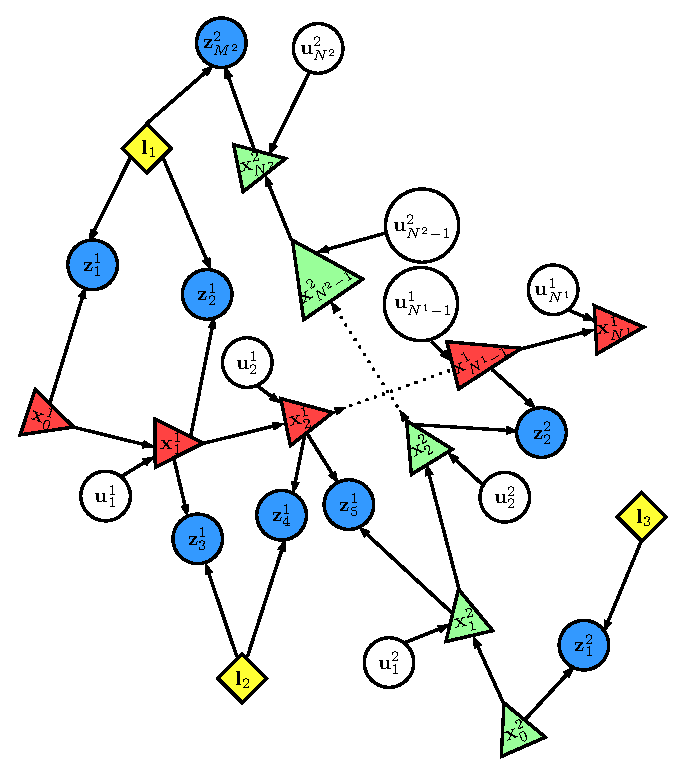
\includegraphics{Chapters/figures2/multi_robot_belief_network}
\caption{A belief network showing direct and indirect encounter in a multi-robot scenario. Robot-robot encounters (direct) are shown by orange arrows and a robot-landmark-robot encounter (indirect) are shown by red arrows.}
\label{fig:multi_bel_net}
\end{figure}
\paragraph{}
In SLAM, loop closures play an important role in significantly improving the overall estimate of all the unknown variables. A loop introduces correlations between the current pose and previously observed landmarks, which themselves are connected to earlier parts of the trajectory. During an update after the loop closure, the belief is propagated all the way through the trajectory to improve the estimate based on the rich set of information obtained. In multi-robot scenario, such belief propagations can be very non-trivial. A robot-robot encounter could give rise to interesting correlations between same portions of map previously visited by both the robots. In such cases, propagating the belief across both the trajectory increases the confidence of the overall map. Figure \ref{fig:multi_bel_net} shows a belief network of a multi-robot encounter. It can be seen that there are two types of interactions - 1) robot-robot and 2) robot-landmark-robot. 
\paragraph{}
Different robots have different sensor models. This is due to variations in the wheel diameter, LIDAR manufacturer \textit{etc}. Upgrading the above symbols to multiple robots, let $X_r = \{\textbf{x}_i^r\}_{r=1,i=0}^{r=R,i=N^r}$, $U_r = \{\textbf{u}_i^r\}_{r=1,i=1}^{r=R,i=N^r}$ and $Z_r = \{\textbf{z}_k^r\}_{r=1,k=0}^{r=R,k=M^r}$ represent the robot's position, control inputs and observations for different robots $r\in 1...R$. The landmarks $L$ need not be redefined as they depend on the environment and not on the number of robots. Then the Equation \ref{eq:lsopt} for multi-robot scenario becomes: 
\begin{multline}
\Theta^*_r = \text{arg} \min_{\Theta_r} \biggl\{ \frac{N^r}{16} \sum_{i=1}^{N^r} \norm{\textbf{x}_{i-1}^r + s_r(\textbf{d}_{i-1}^r, \textbf{d}_i^r) - f_r(\textbf{x}_{i-1}^r,\textbf{u}_i^r)}_{\Xi^r}^2 + \\ \frac{M^r}{16} \sum_{k=1}^{M^r} \norm{\textbf{z}_{k}^r - h_r(f(\textbf{x}_{i-1}^r, \textbf{u}_i^r) + \textbf{w}_p, \textbf{l}_j)}_{\Psi^r}^2 + \\ \frac{1}{4} \text{ln} \biggl( \frac{\mid \Xi^r \mid \mid \Psi^r \mid}{\mid \Lambda^r \mid \sqrt{\mid \Omega^r \mid \mid \Gamma^r \mid}} \biggr) \biggr\}
\label{eq:multilsopt}
\end{multline}
where $f_r(.)$, $s_r(.)$, $h_r(.)$, $w_p^r$, $w_s^r$, $w_m^r$, $\Lambda^r$, $\Omega^r$, $\Gamma^r$ are the process, scan-matching and measurement model, noise and their covariance respectively. Similarly, $\Xi^r = \frac{\Lambda^r+\Omega^r}{2}$ and $\Psi^r = \frac{\Lambda^r+\Gamma^r}{2}$. The optimization is very similar to Extended Kalman Filter (EKF) in \cite{smithekf} except that they are iterated continuously until convergence. 


\section{Solving the Multi-robot Least-Square SLAM}
Both Gauss-Newton and Levenberg-Marquardt proceeds by finding the step value to be added to all the unknowns at every iteration using the approximate linear system at a particular linearization point. To begin with, this linearization point is supplied as initial guess on the decision variables. In other words, we work on the linearized form of the objective function. By using first-order Taylor series approximation on the first term of the objective function in Equation \ref{eq:multilsopt} representing the difference odometry and scan-matching model,
\begin{align}
& \textbf{x}_{i-1}^r + s_r(\textbf{d}_{i-1}^r, \textbf{d}_i^r) - f_r(\textbf{x}_{i-1}^r,\textbf{u}_i^r) \\
\approx & ^0\textbf{x}_{i-1}^r + \delta ^0\textbf{x}^r_{i-1} + \{ s_r(^0\textbf{d}^r_{i-1}, ^0\textbf{d}^r_{i}) + S_r^{i-1}\delta \textbf{d}_{i-1}^r + S_r^{i} \delta \textbf{d}_i^r \} - \{ f_r(^0\textbf{x}_{i-1}^r, \textbf{u}_i^r) + F_r^{i-1}\delta\textbf{x}_{i-1}^r\}\\
= & \{ \delta ^0\textbf{x}^r_{i-1} + S_r^{i-1}\delta \textbf{d}_{i-1}^r + S_r^{i} \delta \textbf{d}_i^r - F_r^{i-1}\delta\textbf{x}_{i-1}^r \} + \{ ^0\textbf{x}_{i-1}^r + s_r(^0\textbf{d}^r_{i-1}, ^0\textbf{d}^r_{i}) - f_r(^0\textbf{x}_{i-1}^r, \textbf{u}_i^r) \} \\
= & \{ \delta ^0\textbf{x}^r_{i-1} + S_r^{i-1}\delta \textbf{d}_{i-1}^r + S_r^{i} \delta \textbf{d}_i^r - F_r^{i-1}\delta\textbf{x}_{i-1}^r \} + \pmb\alpha_i^r
\label{eq:proclin}
\end{align}
where $F_i^{i-1}$ is the Jacobian of the process model with respect to linearization point, $\pmb\alpha_i^r = ^0\textbf{x}_{i-1}^r + s_r(^0\textbf{d}^r_{i-1}, ^0\textbf{d}^r_{i}) - f_r(^0\textbf{x}_{i-1}^r, \textbf{u}_i^r)$ is the difference in odometry and scan-matching prediction and a superscript on the left side of the variable indicate the index number of optimization iteration, a $"0"$ indicates initial guess.
\begin{equation}
F_r^{i-1} := \frac{\partial f_r(\textbf{x}^r_{i-1}, \textbf{u}^r_{i})}{\partial \textbf{x}_{i-1}^r} \bigg\rvert_{^0\textbf{x}_{i-1}^r}
\end{equation}
\begin{equation}
S_r^{i-1} := \frac{\partial s_r(\textbf{d}^r_{i-1}, \textbf{d}^r_{i})}{\partial \textbf{d}_{i-1}^r} \bigg\rvert_{(^0\textbf{d}_{i-1}^r,^0\textbf{d}_{i}^r)}
\end{equation}
\begin{equation}
S_r^{i} := \frac{\partial s_r(\textbf{d}^r_{i-1}, \textbf{d}^r_{i})}{\partial \textbf{d}_{i}^r} \bigg\rvert_{(^0\textbf{d}_{i-1}^r,^0\textbf{d}_{i}^r)}
\end{equation}
The first-order Taylor expansion of the second term in the objective function Equation \ref{eq:multilsopt} scan-matching and measurement model is as follows:
\begin{align}
& \textbf{z}_{k}^r - h_r(f_r(\textbf{x}_{i-1}^r, \textbf{u}_i^r) + \textbf{w}_p, \textbf{l}_j) \\
\approx & \textbf{z}_{k}^r - \{ h_r(f_r(^0\textbf{x}_{i-1}^r, \textbf{u}_i^r), ^0\textbf{l}^r_{j_k}) + H_r^{i_k}\delta \textbf{x}_{i_k}^r + J_r^{j_k} \delta \textbf{l}_{j_k} \} \\
= & \pmb\beta_i^r - \{ H_r^{i_k}\delta \textbf{x}_{i_k}^r + J_r^{j_k} \delta \textbf{l}_{j_k}\}
\label{eq:measlin}
\end{align}
where $H_r^{i_k}$ and $J_r^{j_k}$ is the Jacobian of measurement model with respect to $\textbf{x}^r_{i_k}$ and $\textbf{l}^r_{i_k}$ and $\pmb\beta_i^r = \textbf{z}_{k}^r - h_k(f(^0\textbf{x}_{i-1}^r, \textbf{u}_i^r), ^0\textbf{l}^r_{j_k})$ is the measurement prediction error.
\begin{equation}
H_r^{i_k} := \frac{\partial h_r(\textbf{x}_{i_k}, \textbf{l}_{j_k})}{\partial f(\textbf{x}_{i-1}^r, \textbf{u}_i^r)}.\frac{\partial f_r(\textbf{x}^r_{i-1}, \textbf{u}^r_{i})}{\partial \textbf{x}_{i-1}^r} \bigg\rvert_{(^0\textbf{x}_{i_k}^r,^0\textbf{l}_{j_k}^r)}
\end{equation}
\begin{equation}
J_r^{j_k} := \frac{\partial h_r(\textbf{x}_{i_k}, \textbf{l}_{j_k})}{\partial \textbf{l}_{j_k}^r} \bigg\rvert_{(^0\textbf{x}_{i_k}^r,^0\textbf{l}_{j_k}^r)}
\end{equation}
 
\paragraph{}
Substituting the Taylor approximated linear system formulated in the Equations \ref{eq:proclin} and \ref{eq:measlin} back in the non-linear least squares problem in \ref{eq:multilsopt}:
\begin{multline}
\delta\Theta^*_r = arg \min_{\delta\Theta_r} \biggl\{ \frac{N}{16} \sum_{i=1}^{N} \norm{ G^{i-1}_r\delta ^0\textbf{x}^r_{i-1} + S_r^{i-1}\delta \textbf{d}_{i-1}^r + S_r^{i} \delta \textbf{d}_i^r - F_r^{i-1}\delta\textbf{x}_{i-1}^r + \pmb\alpha_i^r}_\Xi^2 + \\ \frac{M}{16} \sum_{k=1}^{M} \norm{\pmb\beta_i^r - H_r^{i_k}\delta \textbf{x}_{i_k}^r + J_r^{j_k} \delta \textbf{l}_{j_k}}_\Psi^2 + \\ \frac{1}{4} \text{ln} \biggl( \frac{\mid \Xi^r \mid \mid \Psi^r \mid}{\mid \Lambda^r \mid \sqrt{\mid \Omega^r \mid \mid \Gamma^r \mid}} \biggr) \biggr\}
\label{eq:multilinlsopt}
\end{multline}
where $\delta\Theta_r = [\delta X_r;\delta L_r]$ and $\delta\Theta^*_r = [\delta X^*_r;\delta L^*_r]$ is the step size to be added to all the unknown variables towards minimizing the cost function. This now forms a linear least squares problem in $\delta\Theta$. The length of the state vector is given as $n^r = N^r\textbf{d}^r_\textbf{x}+K^r\textbf{d}^r_\textbf{l}$ where $\textbf{d}^r_\textbf{x}$ and $\textbf{d}^r_\textbf{l}$ is the dimension of pose and landmark variables. $G^{i-1}_r = I_{\textbf{d}^r_x\times\textbf{d}^r_x}$ is the identity matrix of size $\textbf{d}^r_x$. The $\delta\textbf{d}^r_{i-1}$ and $\delta\textbf{d}^r_{i}$ terms are not added to the state vector as they are estimated as a part of the scan-matching process. See [Appendix] [Appendix 2] for details. The covariance terms weighting the squared norms could be removed by multiplying the Jacobians with the transpose of inverse square-root of the covariance:
\begin{equation}
\norm{\textbf{e}}^2_\Sigma := \textbf{e}^{\top}\Sigma^{-1}\textbf{e} = (\Sigma^{-T/2}\textbf{e})^{\top}(\Sigma^{-T/2}\textbf{e}) = \norm{\Sigma^{-T/2}\textbf{e}}^2
\label{eq:simplifymaho}
\end{equation}
By using the relation \ref{eq:simplifymaho} in Equation \ref{eq:multilinlsopt} we can simplify it to group all the model specific Jacobians into single large Jacobian $A_r\in\mathbb{R}^{m\times n}$ where $m$ is the total number of input measurements scaled to dimension of each measurement. The constants in the objective function including $\pmb\alpha_i^r$, $\pmb\beta_i^r$ and the  natural logarithm term can be grouped to form $\textbf{b}^r \in \mathbb{R}^m$. We obtain a over-determined system of linear equations that require inverting a huge matrix to find the solution:
\begin{equation}
\delta\Theta^*_r = arg \min_{\delta\Theta_r}\norm{A_r\delta\Theta_r - \textbf{b}^r}^2
\label{eq:multisimplifiedopt}
\end{equation}
The above optimization can be minimized by setting the derivative equal to zero. With the assumption that we begin at a good linearization point (good initial guess) we are bound to slide into the global minima. 

\subsection{Incremental Optimization}
An optimization problem is often supplemented by an initial guess for the decision variables. In our case, we have to supply the initial guess for the variables to be estimated whose error will then be iteratively reduced based on the measurements. However, one important aspect to be worried about is the source of the initial guess. Modern robots are mostly accompanied with more sensors than necessary for localization, and hence one of them can be utilized as the source for initial guess. But if SLAM is done as a batch process with a fixed lag and not at real-time this again becomes a problem. This is because, sensors like odometry encoder, LIDAR and Inertial Measurement Units (IMU) are very good only at providing a local estimate between nearly successive pose frames but drifts away significantly when forward integrated continuously. Figure \ref{fig:dr_vs_slam} shows an example comparison between a robot's trajectory generated from dead reckoning odometry and SLAM reconstruction. Thus, incremental optimization is beneficial in several ways that include:
\begin{figure}
\centering
\begin{minipage}{.5\textwidth}
  \centering
  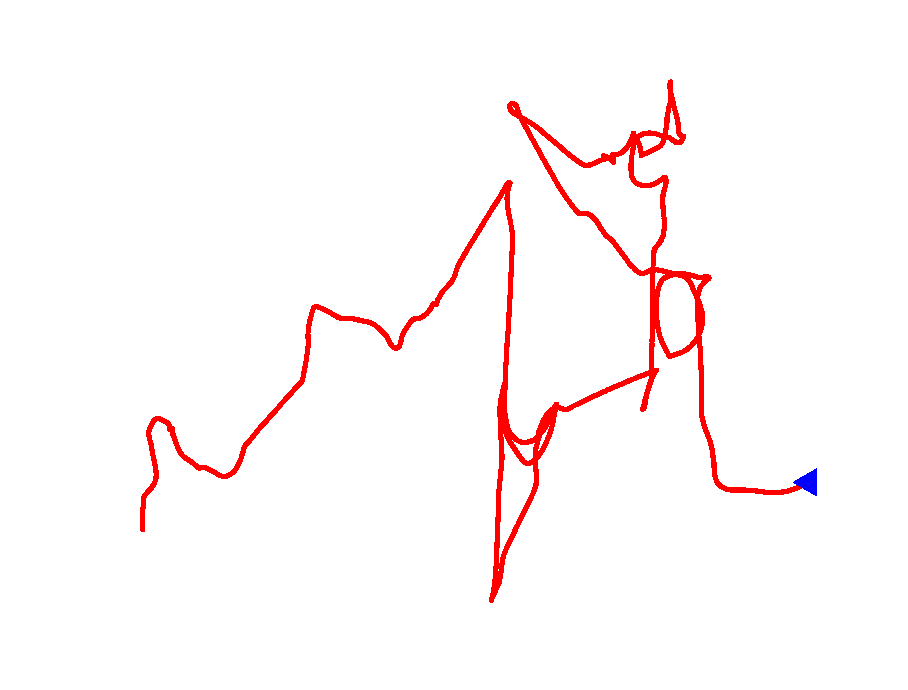
\includegraphics[width=\textwidth]{Chapters/figures2/dead_reckoning}
  %\caption{A subfigure}
  %\label{fig:sub1}
\end{minipage}%
\begin{minipage}{.5\textwidth}
  \centering
  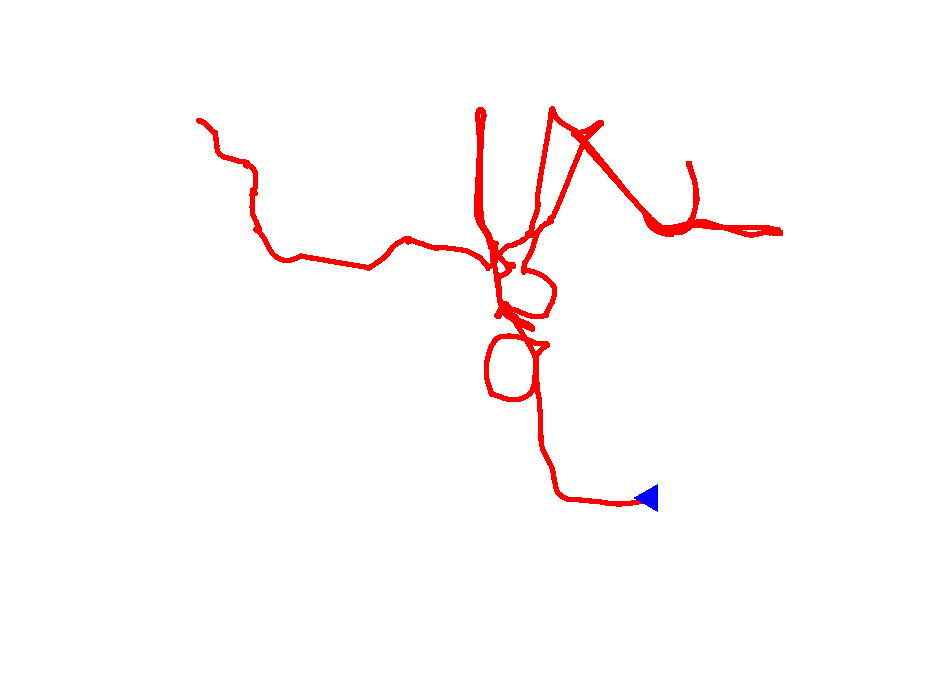
\includegraphics[width=\textwidth]{Chapters/figures2/slam_result}
  %\caption{A subfigure}
  %\label{fig:sub2}
\end{minipage}
\caption{Left: Trajectory obtained by just forward integrating the odometry provided by robot. Right: Trajectory reconstructed after batch SLAM. It can be seen that the plain odometry trajectory looks same as the reconstructed trajectory at the beginning (blue triangle) but starts drifting away due to integral error.}
\label{fig:dr_vs_slam}
\end{figure}
\begin{enumerate}
\item Easier to provide an accurate initial guess based on local sensor information as we have an optimized estimate for variables processed so far. 
\item A good initial guess means that it is close to the optimal solution and saves a lot of optimization time and iterations.
\item A good initial guess also significantly reduces the probability of getting trapped in a local minima. For example, in Figure \ref{fig:dr_vs_slam}, the dead-reckoning odometry trajectory as an initial guess for a batch SLAM optimizer is far away from the optimal solution and may suffer local minima. 
\item Finally, an incremental system gives optimal estimates on the fly and is real-time.
\end{enumerate}
For our purpose, we use ISAM2 \cite{kaessisam2} as the underlying optimization algorithm.

\subsubsection{Jacobian Decomposition} 
This is a well known material but discussed mainly to differentiate linear algebra algorithms with graph theoretic view in the next section. A detailed study is available in the standard textbook \cite{golubmatrixbook}. Matrix decomposition is a very common technique in mathematics and engineering disciplines to factorize the matrix into product matrices so as to arrive at the solution faster than pure inversion. Among several methods available, Cholesky, QR and LDL \cite{golubmatrixbook} decomposition are the ones commonly used by the SLAM community. The Jacobian matrix $A_r$ in Equation \ref{eq:multisimplifiedopt} has a column for every variable being estimated of size $n$ and a row for every sensor measurement of size $m$. It is a very sparse matrix owing to the fact that different measurements are recorded at every pose variable and every measurement measures no more than a few pose variables. As there are multiple sensors, total number of measurements are very large compared to number of variables, i.e. $m \gg n$. With respect to time complexity, both Cholesky and QR factorization require $\mathcal{O}(mn^2)$ operations for dense matrices when $m \gg n$. But for dense and sparse matrices, in practice, we have seen that both Cholesky and LDL factorization outperform QR factorization at least by a factor of 2. However, mathematical tools from linear algebra and graph theory literature like Gram-Schmidt orthogonalization and Householder reflections for QR decomposition along with Givens rotations \cite{golubmatrixbook} for incremental update of the square-root information matrix $R_r$ make QR decomposition as the most suitable choice for our purpose. Also, QR decomposition works directly on the Jacobian matrix $A_r$ unlike Cholesky which needs the information matrix, $\mathcal{I} = {A_r}^{\top}A_r$ to be computed. It is also more accurate and numerically stable compared to Cholesky decomposition. The $Q_r$ matrix is orthogonal and is usually not formed as a part of factorization. The QR factorization of the Jacobian matrix $A_r$ is:
\begin{equation}
A_r = Q_r \begin{bmatrix}
R_r \\
0
\end{bmatrix}
\end{equation}
Applying this factorization to the multi-robot linearized least-squares problem \ref{eq:multisimplifiedopt}:
\begin{align}
\norm{A_r\Theta-\textbf{b}^r} = & \norm{Q_r \begin{bmatrix}
R_r \\
0
\end{bmatrix}\Theta_r - \textbf{b}^r}^2 \\
= & \norm{Q_r^{\top}Q_r\begin{bmatrix}
R_r \\
0
\end{bmatrix}\Theta_r - Q_r^{\top}\textbf{b}^r}^2 \\
= & \norm{\begin{bmatrix}
R_r \\
0
\end{bmatrix}\Theta_r - \begin{bmatrix}
\textbf{d}^r \\
\textbf{e}^r
\end{bmatrix}}^2 \\
= & \norm{R_r\Theta_r - \textbf{d}^r}^2 + \norm{\textbf{e}^r}^2
\label{eqn:qrlsopti}
\end{align}
where $R_r$ is the upper triangular square-root information matrix or square-root factor obtained using QR factorization, $Q_r^{\top}\textbf{b}^r = [\textbf{d}^r; \textbf{e}^r]$, $\textbf{d}^r \in \mathbb{R}^n$, $\textbf{e}^r \in \mathbb{R}^{m-n}$ and $R_r^{\top}R_r = A_r^{\top}A_r$. For the above Equation \ref{eqn:qrlsopti} to attain minimum, $R_r\Theta_r $ should be equal to $\textbf{d}^r$. This leaves the residual of the least squares problem given by $\norm{\textbf{e}^r}^2$. Since $R_r$ is upper triangular, back-substitution is trivial and the estimate $\delta\Theta_r$ is added to the linearization point to update and proceed with the next iteration.

\section{Foundations of Matrix and Graphs}
A major key to the improving performance of pose graph based SLAM algorithms is rooted in tiny numerical optimizations developed over time. One has to analyze the deep connections between Linear Algebra and Graph Theory in conjunction with SLAM algorithms to understand this fact better. Due to the nature of SLAM problem, we specifically deal with sparse graphs and matrices. Both sparse linear algebra and graph theory has flourished over the past four decades with each being critical to other \cite{graphandla}. This section gives a brief grounding of terminologies frequently used in the upcoming chapters and then examines the relationship between matrices and graphs. 

\subsection{Graph Theory Terminology}
\textbf{Definition:} A \textbf{graph} $G=(V,E)$ is a collection $V$ of vertices and $E \subset V \times V$ of edges. Informally, we think of the edges as linking the pairs of vertices that they correspond to, and typically represents graphs by drawings in which we connect the endpoints by a curve.
\paragraph{Glossary of Terms:}
\begin{itemize}
\item A graph is \textbf{simple} if every edge links a unique pair of distinct vertices. 
\item A graph is \textbf{bipartite} if the vertex set can be partitioned into two sets $V_1 \cup V_2$ such that edges only run between $V_1$ and $V_2$.
\item A \textbf{clique} on $n$ vertices, denoted $K_n$, is the $n$-vertex graph with all $\bigl( _2^n \bigr)$ possible edges.
\item A \textbf{complete graph} on $n$ vertices, denoted $K_n$, is the $n$-vertex graph with all $\bigl( _2^n \bigr)$ possible edges.
\item A graph is \textbf{connected} if there is a path between every pair of distinct vertices.
\item A \textbf{cycle} is a path for which the first and last vertices are the same.
\item A \textbf{chord} is an edge that is not part of the cycle but connects two vertices of the cycle.
\item A \textbf{chordal graph} is one in which all cycles of four or more vertices have a chord.
\item The \textbf{degree} $d(v)$ of a vertex $v$ is the number of edges that are incident to $v$.
\item We say that an edge $e$ is \textbf{incident} to a vertex $v$ if $v$ is an endpoint of $e$.
\item A \textbf{path} is a sequence of distinct, pairwise-adjacent vertices.
\item A graph is \textbf{planar} if it is possible to draw it in the plane without any crossing edges.
\item A \textbf{tree} is a connected graph with no cycles.
\item A \textbf{subgraph} of a graph $G$ is another graph formed from a subset of the vertices and edges of $G$. The vertex subset must include all endpoints of the edge subset, but may also include additional vertices.
\item A \textbf{supergraph} is a graph formed by adding vertices, edges, or both to a given graph. If $H$ is a subgraph of $G$, then $G$ is a supergraph of $H$.
\item A \textbf{connected component} (or just \textbf{component}) of an undirected graph is a subgraph in which any two vertices are connected to each other by paths, and which is connected to no additional vertices in the supergraph.
\end{itemize}

\subsection{Factor Graph and Bayes Tree}
A formal introduction of factor graphs \cite{factorgraph} and Bayes tree \cite{kaessbayestree} is presented below. I will also provide details on how the formulations made in this subsection relate to ones derived previously. This section might slightly abuse the usage of symbols and hence should not be confused with the usage in the previous sections.

\subsubsection{Factor Graph}
A factor graph is a bipartite graph $\mathcal{G} = (\mathcal{C}, \Theta, \mathcal{E})$ with two node types: factor nodes $c^p \in \mathcal{C}$ and variable nodes $\theta^q \in \Theta$. Edges $e^{pq} \in \mathcal{E}$ are always between factor nodes and variable nodes. A factor graph $\mathcal{G}$ represents the factorization of a function: 
\begin{equation}
c(\Theta) = \prod_p c^p(\Theta_p)
\end{equation}
where $\Theta^p$ is the set of variables $\theta^q$ adjacent to the factor $c^p$. The independence relationship between the factors and variables are encoded by the edges $e^{pq}$. Every factor $c^p$ is a function of variables contained in $\Theta^p$. Assuming Gaussian measurement models:
\begin{equation}
c^{pq} \propto \text{exp}\biggl( -\frac{1}{2} \norm{\mathcal{H}^p(\Theta^p)-\mathcal{Z}^p}^2_{\Sigma^p} \biggr)
\end{equation}
The above equation is a consolidation of detailed objective function listed in \ref{eq:multilinlsopt} to minimize the net difference between prediction $\mathcal{H}^p(\Theta^p)$ and measurement $\mathcal{Z}^p$ weighted by the covariance $\Sigma^p$. 

\subsubsection{Bayes Network}
A Bayes net is obtained as an intermediate structure when \textit{eliminating} a factor graph into Bayes tree. Eliminating a factor graph into a Bayes tree uses a variable elimination procedure which has roots dated 2000 years ago in Chinese and Indian literature \cite{oldchina}. In the modern times, variable elimination was first implemented by C. F. Gauss in 1809 \cite{gauss}. Factor graphs elimination is done using bipartite elimination game that was proposed by Heggernes \textit{et al.} \cite{heggernesordering}. Variable elimination is a procedure of expressing a variable in terms of other, one at a time based on sequence given by variable ordering. On eliminating every variable a corresponding node is introduced in the Bayes net that has conditional variables directed towards it. The conditional variables are the independent variables used to express the eliminated variable at every iteration. This process continues until all the variables are eliminated in the factor graph. Thus, the structure of the Bayes net depends on the choice of variable ordering and any operation carried out on it is specific to that ordering. The pseudo code for a quick understanding of eliminating the factor graph into Bayes net is present in \cite{kaessbayestree}
\label{sss:bayes_net_intro}

\subsubsection{Bayes Tree}
The Bayes net resulting from the elimination of variables is chordal. This chordal graph can be converted into a Bayes tree by identifying the cliques in the graph. This was first intoduced by Kaess \textit{et al.} in \cite{kaessbayestree}. A Bayes tree is a directed tree where the nodes represent cliques of the underlying chordal Bayes net. In this respect, Bayes trees are similar to clique trees, but a Bayes tree is directed and is closer to a Bayes net in the way it encodes a factored probability density. Every chordal Bayes net can be transformed into a tree by discovering its cliques. Discovering cliques in chordal graphs is done using the maximum cardinality search algorithm by Tarjan and Yannakakis \cite{fgtobn}, which proceeds in the \textit{reverse elimination order} to discover cliques in the Bayes net. In this regard, as a Bayes tree is generated out of the Bayes net, the structure of the Bayes tree is also specific to the variable ordering. From the Bayes tree it is not possible to retrieve the order in which the variables were measured. 

\subsection{Matrix vs. Graph}
In the following chapters, this thesis revolves around two main types of graphical models and a type of tree data structure. They are central in understanding the contributions of the work and gaining sufficient intuition on how they are related to their equivalent matrix representations is imperative. The two types of graphical models include factor graphs \cite{factorgraph} and Bayesian Network. Bayes Tree \cite{kaessbayestree} is the tree data structure used widely in this work. 

\subsubsection{Jacobian vs. Factor Graph}
The measurement Jacobian $A_r$ is the matrix of the factor graph associated with SLAM. This statement can be understood in two stages: 
\begin{enumerate}
\item Every block of $A_r$ corresponds to one term in the least-squares criterion \ref{eq:multilinlsopt}, either a landmark measurement or an odometry/scan-matching  constraint, and every block-row corresponds to one factor in the factor graph. Within each block-row, the sparsity pattern indicates which unknown poses and/or landmarks are connected to the factor. Hence, the block-structure of A corresponds exactly to the adjacency matrix of the factor graph associated with SLAM.
\item At the scalar level, every row $A^j$ in A corresponds to a scalar term $\norm{A^j_r\delta - \textbf{b}^r}^2_2$ in the sparse matrix least squares criterion:
\begin{equation}
\norm{A_r\delta - \textbf{b}}^2_2 = \sum_j \norm{A^j_r\delta - \textbf{b}^r}^2_2
\end{equation} 
The reordering is not done across all the scalar parts of the pose and landmark variables as done by the standard linear algebra literature. But for our case, such a fine and granular ordering is not needed for two reasons 1) We would then be operating on a larger matrix and hence takes longer time for finding a variable ordering. 2) A single pose constraint or landmark measurement introduces a block and all the scalars in them are generally non-zero. So it is better to operate on these blocks rather than those fine scalar variables \cite{dellaertsam}.
\end{enumerate}

\subsubsection{Square-root Information vs. Bayes Network}
The square-root information matrix is more or less the adjacency matrix of the Bayes net. Since it is a directed graph, the adjacency matrix is not going be symmetric. Nevertheless, the square-root factor $R_r$ is upper triangular and not a symmetric matrix. The arrows pointing towards any node in the Bayes net denoting the variables on which the node is conditioned upon, is analogous to a non-zero present other than the main diagonal in the row corresponding to that node. The Bayes net also indicates conditional independence relationship between variables as that of a factor graph. But the relation follows a causal direction implied by the choice of variable ordering. By definition, although a Bayes net does not have any cycles they contain loops. Storing and updating the Bayes net by attaching new factors and variables to a node in these loops is intractable because 1) Changes to the direction of arrows within a clique is not understood \cite{kaessbayestree} 2) Additional variables that get affected is not elegantly traceable. 

\subsubsection{Square-root Information vs. Bayes Tree}
\label{sss:r_vs_bt}
One of the finest outcomes from The Borg Lab at Georgia Tech was incremental smoothing and mapping using the Bayes tree (ISAM2) \cite{kaessisam2}. The increase in performance over other pose graph SLAM solutions comes from using the Bayes tree \cite{kaessbayestree} to represent the cliques of the square-root factor or the Bayes net in the incremental smoothing and mapping (iSAM). Updating the square root factor with a new measurement removes its upper triangularity. It is made upper triangular again by using Givens rotations \cite{golubmatrixbook}. During this process, the new measurement row is multiplied with the Givens rotation matrix producing new non-zeros replacing zeros in the upper triangle. The pattern in which these non-zeros are generated is unintuitive and was not understood in the matrix form. The new non-zero elements that are created during variable elimination is referred as fill-in. These blocks of non-zeros relate to the cliques in the Bayes tree. The row in $R_r$ corresponding to the first eliminated frontal variable of any clique has non-zeros in the positions corresponding to the rest of the variables of that clique. However, by representing the square root factor $R_r$ as a Bayes tree an independence relation conditioned on the \textit{variable ordering} is established across variables that allows us to find the subset of variables that gets affected on adding a new measurement. This also led to an interesting concept of just-in-time fluid relinearization that updates the linearization point incrementally and efficient access to marginal covariances \cite{kaesscovariance}. 

\subsection{Factor Graph $\rightarrow$ Bayes Network $\rightarrow$ Bayes Tree}
\label{ss:fg_to_bn_to_bt}
Despite the attempts to simplify the understanding of relevant matrix-graph relation, one may still wonder how to eliminate any arbitrary factor graph into a Bayes net and in turn convert a Bayes net into a Bayes tree. This portion of research has spanned over several decades and intersects different areas of study including sparse linear algebra, graph theory, probabilistic and statistical inference, finite element analysis and numerical analysis. It is therefore beyond the scope of this piece of work to provide a step-by-step explanation. However, a brief visual treatment is attempted to expedite the process of understanding in Figure \ref{fig:fg_to_bn} and \ref{fig:bn_to_bt}. Some seminal works that could be referred include \cite{chordalcliqueintro, kaessbayestree, fgtobn, heggernesordering, oldchina, cowellprobabilistic}
\begin{figure}
\centering
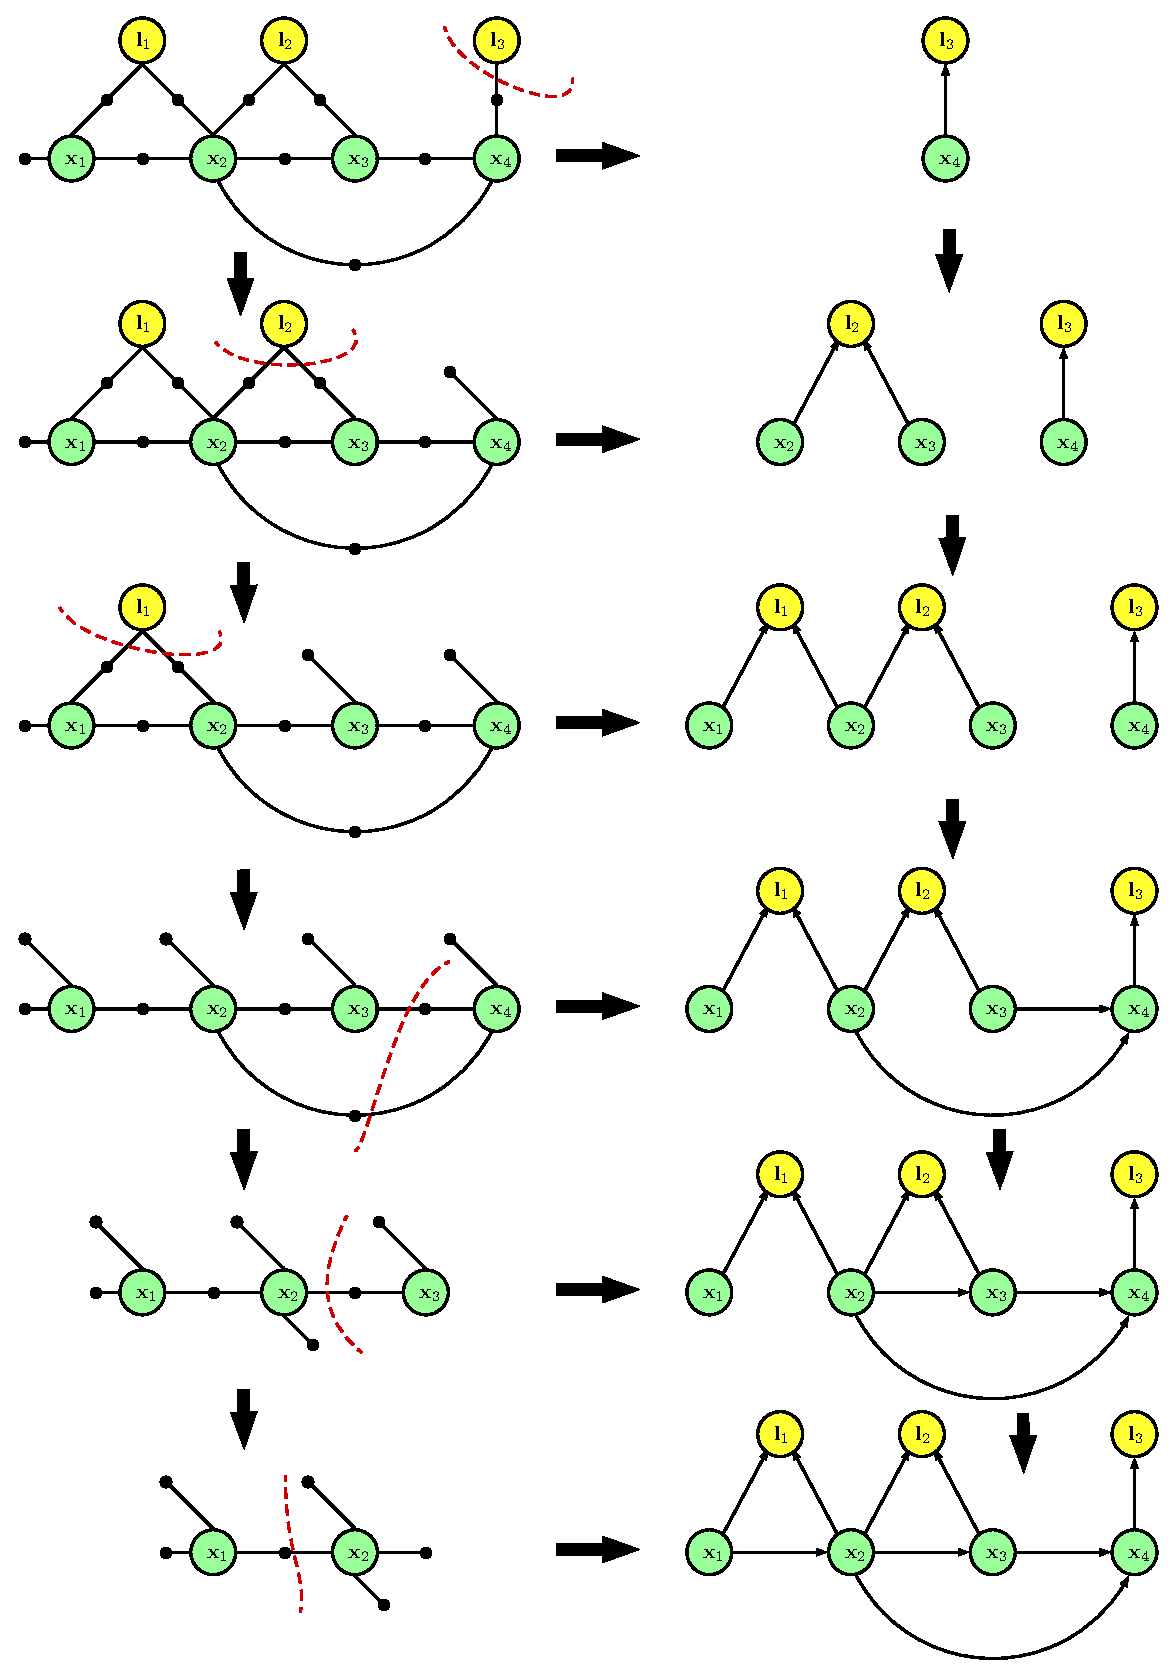
\includegraphics[width=\textwidth]{Chapters/figures2/from_fg_to_bn}
\caption{Eliminating a factor graph into a Bayes net. The elimination order used for converting is $O = [l_3, l_2, l_1, x_4, x_3, x_2, x_1]$. The vertex of the factor graph that is removed at every step is shown by a red dotted separator. The horizontal arrows indicate the equivalent Bayes net on removing a factor graph vertex. The vertical arrows point the progress within the factor graph and Bayes net.}
\label{fig:fg_to_bn}
\end{figure}
\begin{figure}
\centering
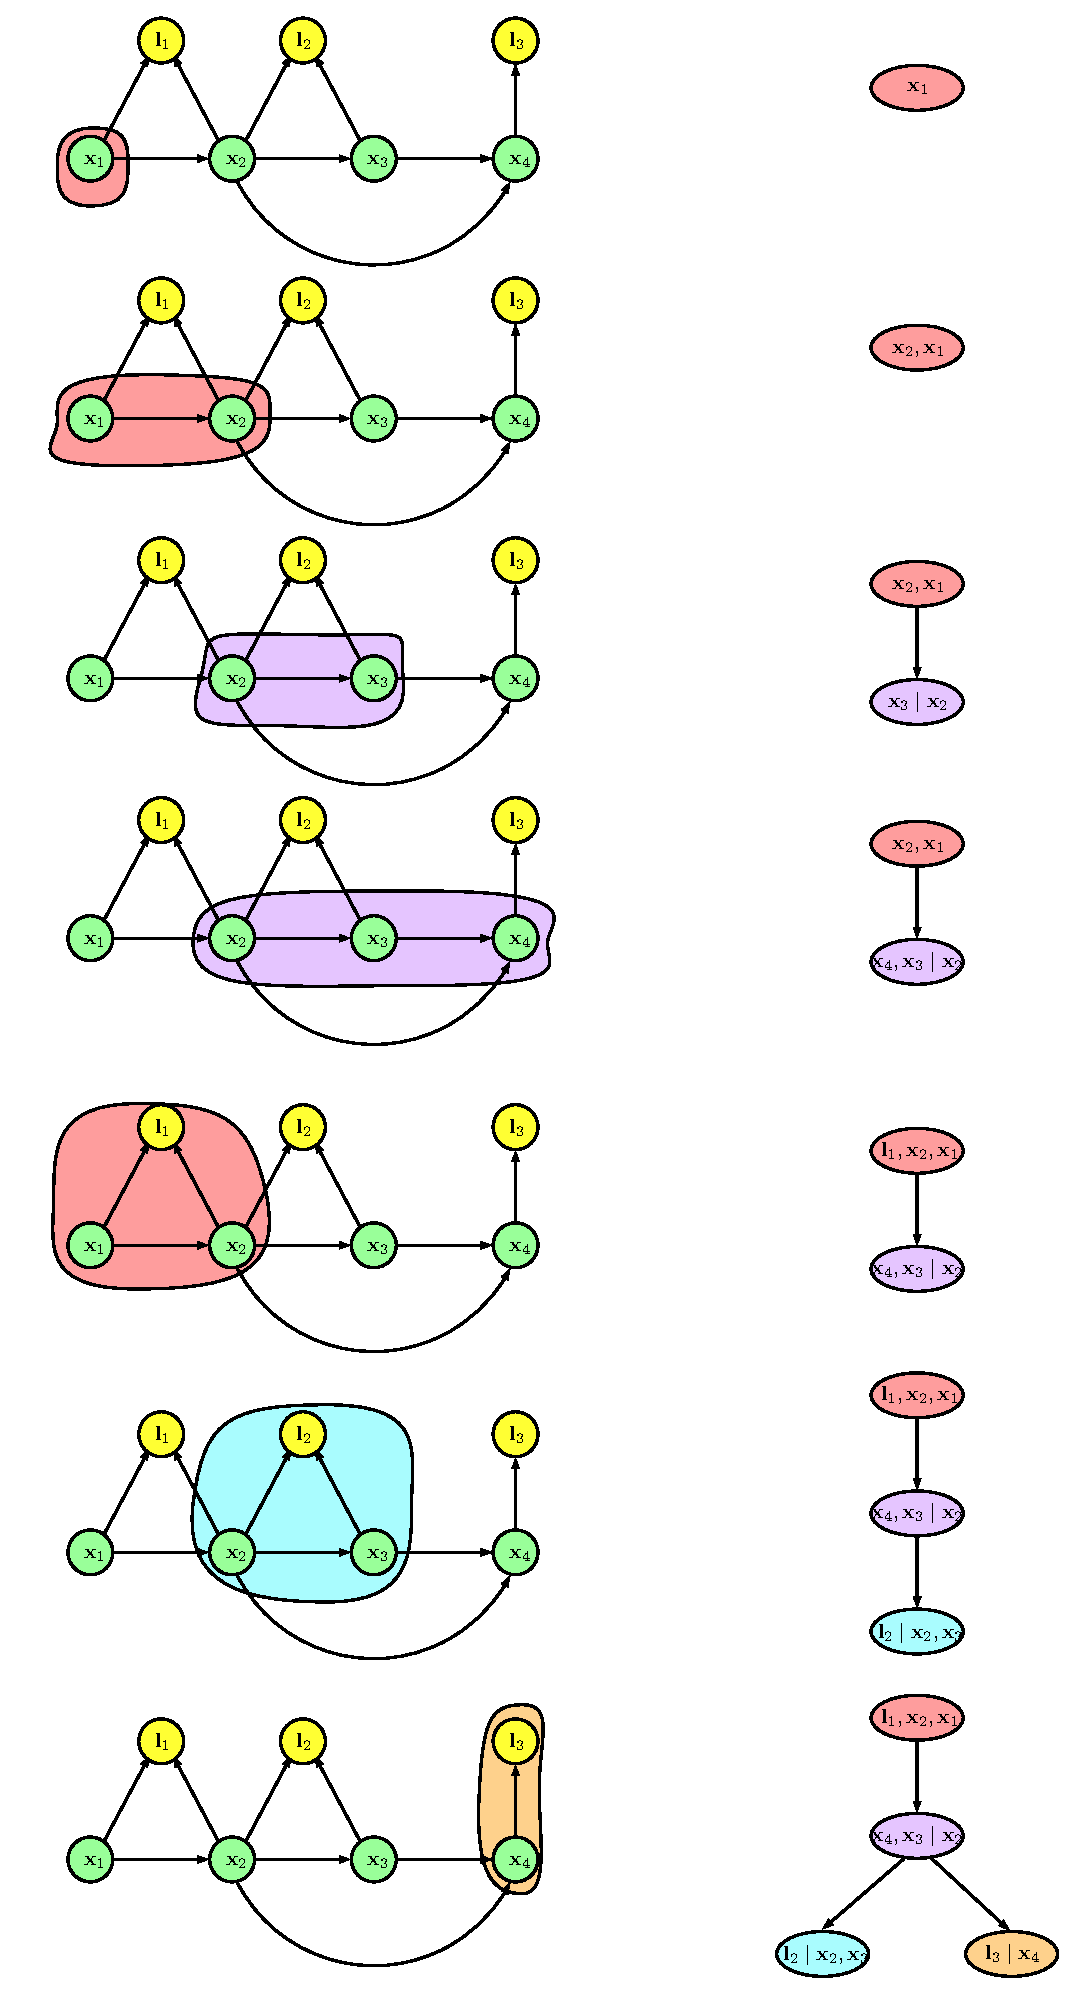
\includegraphics[width=\textwidth,height=\textheight]{Chapters/figures2/from_bn_to_bt}
\caption{Converting a Bayes net into a Bayes tree by clique factorization. The bubble around the node(s) in the Bayes net indicate the cliques found at every iteration based on reverse elimination ordering $x_1, x_2, x_3, x_4, l_1, l_2, l_3$. The color of the bubble denotes the node being added to the same colored clique.}
\label{fig:bn_to_bt}
\end{figure}

\section{Variable Reordering}
This is the most important section of this chapter as it is the gateway towards the set of contributions. The most dramatic improvement in performance comes from choosing a good variable ordering when factorizing a matrix. This variable ordering is used by the graph theoretic algorithm called \textit{variable eliminiation}, in which each variable is expressed in terms of other variables based on the order of elimination. The order in which the variables are eliminated has a large impact on the running time and storage of matrix factorization algorithms such as QR and Cholesky factorization. Finding an optimal ordering is an NP-complete problem \cite{orderingnphard}, but there are numerous ordering heuristics and approximate algorithms that perform well on general problems \cite{colamd, heggernesordering}. While a great deal of improvement in terms of storage and time complexity is obtained by using these general purpose orderings, yet another order-of-magnitude improvement is obtained by exploiting the structure of SLAM problem. Ordering the variables depending on the nature and structure of the problem is not unprecedented and has been a trend in linear algebra \cite{latrend}. It is therefore valid to believe that more efficient and sophisticated algorithms can be developed by viewing the problem as one of the computation on a SLAM pose graph. While a large body of work is available for delivering a comprehensive or esoteric explanation about the need for variable ordering, in my thesis, I will provide a quick overview using a practical example and simple language.

\subsection{Variable Ordering for QR Factorization}
Given a variable ordering $O$, the QR factorization using Gram-Schmidt process works as follows: At every iteration, a column vector as per the sequence in variable ordering is orthogonalized with respect to all the previously orthogonalized column vectors (the first column vector is taken as-is). These orthogonalized vectors are unit normalized and stacked horizontally to form the orthonormal $Q$ matrix. The order of columns in $Q$ follows the same ordering as $O$. Given a full column rank matrix $A=[\mathbf{a}_{1},\cdots ,\mathbf{a} _{n}]$ with inner product defined as $\langle \mathbf {v} ,\mathbf {w} \rangle =\mathbf {v} ^{\top }\mathbf {w}$ then $\textbf{u}_k$ is:
\begin{align}
 \mathbf{u}_k &= \mathbf{a}_k-\sum_{j=1}^{k-1}\mathrm{proj}_{\mathbf{u}_j}\,\mathbf{a}_k,
  &\mathbf{e}_k &= {\mathbf{u}_k\over\|\mathbf{u}_k\|} & \forall \ k &= 1 \cdots n 
\end{align}
where
\begin{equation}
\mathrm {proj} _{\mathbf {e} }\mathbf {a} ={\frac {\left\langle \mathbf {e} ,\mathbf {a} \right\rangle }{\left\langle \mathbf {e} ,\mathbf {e} \right\rangle }}{\mathbf {e} }
\end{equation}
Then $Q$ is given as,
\begin{equation}
Q=\left[\mathbf {e} _{1},\cdots ,\mathbf {e} _{n}\right]
\label{eq:Qshort}
\end{equation}
As $Q$ is an orthonormal matrix $Q^{\top}Q = 1$. The $R$ matrix of QR factorization is now obtained using the below step:
\begin{equation}
\begin{matrix}
R = Q^{\top }Q\,R = Q^{\top } A;
\end{matrix}
\end{equation}
Expanding the value of $R$ with $A=[\mathbf{a}_{1},\cdots ,\mathbf{a} _{n}]$ and Equation \ref{eq:Qshort}:
\begin{equation}
R={\begin{pmatrix}\langle \mathbf {e} _{1},\mathbf {a} _{1}\rangle &\langle \mathbf {e} _{1},\mathbf {a} _{2}\rangle &\langle \mathbf {e} _{1},\mathbf {a} _{3}\rangle &\ldots \\0&\langle \mathbf {e} _{2},\mathbf {a} _{2}\rangle &\langle \mathbf {e} _{2},\mathbf {a} _{3}\rangle &\ldots \\0&0&\langle \mathbf {e} _{3},\mathbf {a} _{3}\rangle &\ldots \\\vdots &\vdots &\vdots &\ddots \end{pmatrix}}
\label{eq:R}
\end{equation}
The inner product $\langle \mathbf{e_i}, \mathbf{a_j} \rangle = 0; \ \forall \ j < i$ because at every iteration $k$, $\mathbf{e}_k$ is the orthogonalized version of $\mathbf{a}_k$ with $\mathbf{e}_l; \ \forall \ l < k$. To retain the sparsity of the square root factor it is necessary to have as many inner products, $\langle \mathbf{e_i}, \mathbf{a_j} \rangle$, equalling 0 as possible. The inner product of two vectors are zero if they are orthogonal or if the intersection of their components forms a nullset. The latter is a specific case of the former. From the general representation of $R$ in Equation \ref{eq:R} it can be seen that, the lower the value of subscript of $\mathbf{e}$ higher is its presence. So lesser the dimension of a $\mathbf{e}_i$ for lesser values of $i$ higher is the probability that it does not share a component with $\mathbf{a}_j$. The vector $\mathbf{e}_i$ with the lowest dimension corresponds to a column $i$ in $A$ with maximum zeros. In other words, as the columns of the Jacobian matrix $A$ is same as the nodes of the factor graph, the previous statement refers to node with the lowest degree. Based on the above explanation, an example matrix and its equivalent factor graph with two different orderings are factorized to show the difference in the non-zero pattern in $R$.
\paragraph{}
Consider a measurement Jacobian A as given below with the column number annotated on top of each column:
\[ 
A = 
\begin{blockarray}{cccccc}
1 & 2 & 3 & 4 & 5 & \\
\begin{block}{(ccccc)c}
2 & 0 & 0 & 4 & 0 & \\
0 & 4 & 8 & 0 & 0 & \\
0 & 0 & 1 & 0 & 1 & \\
1 & 0 & 0 & 0 & 10 & \\
0 & 0 & 6 & 6 & 0 & \\
\end{block}
\end{blockarray}
\]
Let us assume the column elimination ordering as $O = [x_2, x_3, x_4, x_1, x_5]$. The transformed matrix $A^O$ based on the ordering $O$ and the structure of $R^O$ on factorizing the transformed matrix is given below:
\begin{figure}[H]
\begin{minipage}{0.5\textwidth}
\centering
\[ 
A^O = 
\begin{blockarray}{cccccc}
x_2 & x_3 & x_4 & x_1 & x_5 & \\
\begin{block}{(ccccc)c}
0   &   0     & 4     & 2     & 0 & \\
4   &   8     & 0     & 0     & 0 & \\
0   &   1     & 0     & 0     & 1 & \\
0   &   0     & 0     & 1    & 10 & \\
0   &   6     & 6     & 0     & 0 & \\
\end{block}
\end{blockarray}
\]
\end{minipage}
\begin{minipage}{0.5\textwidth}
\centering
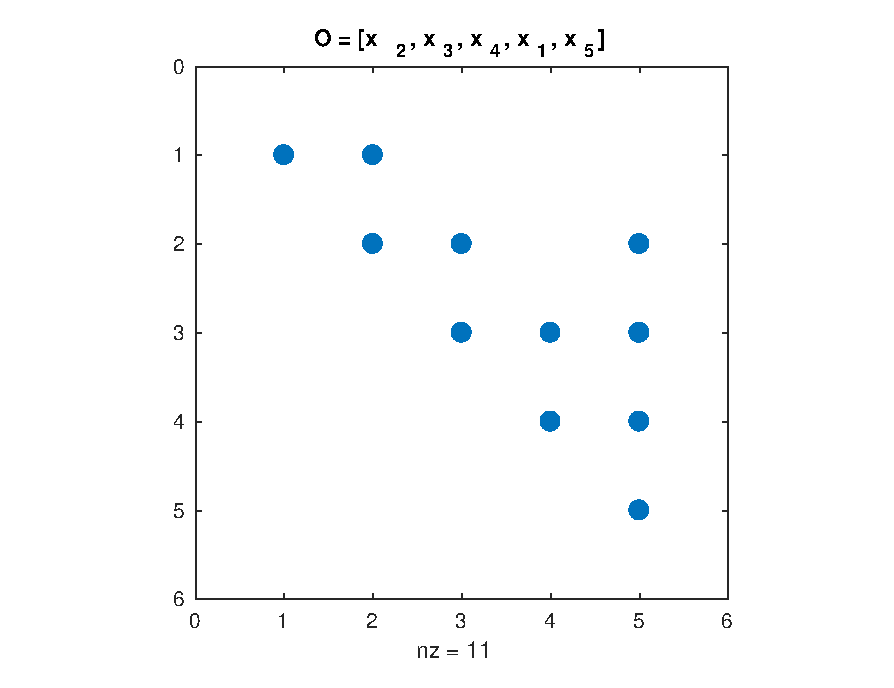
\includegraphics[width=\textwidth]{Chapters/figures2/sample_R_good}
\end{minipage}
\caption{Left: Matrix in which the lower degree node $x_2$, $d(x_2)=1$, is ordered before the higher degree node 3, $d(x_3)=3$. The structure of square root factor $R^O$ with 11 non-zero elements.}
\label{fig:good_ordering}
\end{figure}
The above ordering is also performed in the factor graph and factorized into a Bayes tree as shown in Figure \ref{fig:good_ordering_graph}
\begin{figure}[H]
\centering
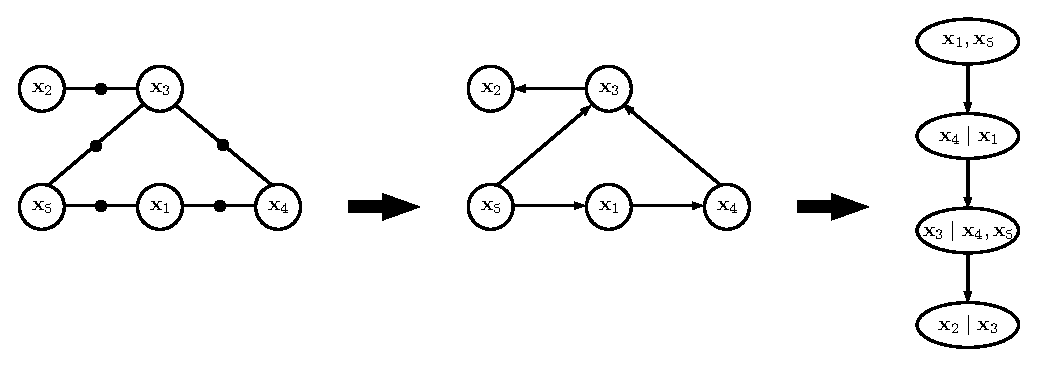
\includegraphics[width=\textwidth]{Chapters/figures2/good_ordering}
\caption{Eliminating a factor graph into a Bayes net and in turn into a Bayes tree. A good ordering has resulted in smaller cliques or reduced fill-in.}
\label{fig:good_ordering_graph}
\end{figure}
\paragraph{}
Whereas if the matrix is ordered by placing the vector with highest dimension or the node with the highest degree at the first place, for example $O = [x_3, x_4, x_1, x_2, x_5]$, then the structure of square root factor $R^O$ is as follows:
\begin{figure}[H]
\begin{minipage}{0.5\textwidth}
\centering
\[ 
A^O = 
\begin{blockarray}{cccccc}
x_3 & x_4 & x_1 & x_2 & x_5 & \\
\begin{block}{(ccccc)c}
0  &   4  &   2  &   0  &   0 & \\
8  &   0  &   0  &   4  &   0 & \\
1  &   0  &   0  &   0  &   1 & \\
0  &   0  &   1  &   0  &  10 & \\
6  &   6  &   0  &   0  &   0 & \\
\end{block}
\end{blockarray}
\]
\end{minipage}
\begin{minipage}{0.5\textwidth}
\centering
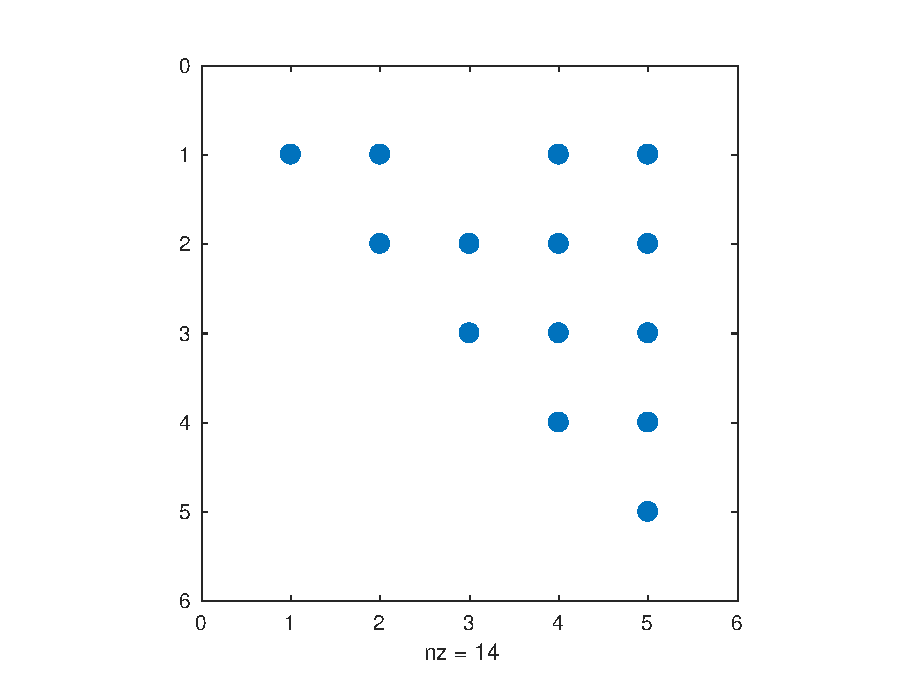
\includegraphics[width=\textwidth]{Chapters/figures2/sample_R_bad}
\end{minipage}
\caption{Left:Jacobian matrix with highest degree variable $x_3$ of degree $d(x_3)=3$ in the first place. Right: The square-root factor with higher fill-in when compared the ordering $O = [x_2, x_3, x_4, x_1, x_5]$. Although the increase in non-zeros is only 4, it is very large given the original fill-in and the size of the matrix.}
\label{fig:bad_ordering}
\end{figure}
Applying the above ordering in the factor graph yields a Bayes tree with a large clique representing the fill-in as shown in Figure \ref{fig:bad_ordering_graph},
\begin{figure}[H]
\centering
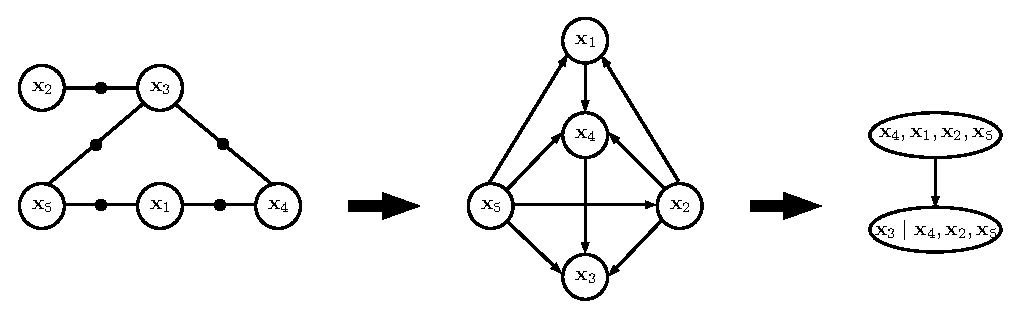
\includegraphics[width=\textwidth]{Chapters/figures2/bad_ordering}
\caption{Eliminating a factor graph into a Bayes net and in turn into a Bayes tree. Eliminating nodes of higher degree at the beginning has resulted in larger cliques or high fill-in.}
\label{fig:bad_ordering_graph}
\end{figure}

Although ordering the variables based on the minimum degree seems to work for small examples like the above, it quickly plummets in terms of time and storage efficiency as the degree of the remaining nodes get affected on eliminating a variable. This change in the degree has to be tracked separately and accounted in the algorithm. Several previous works have showed that keeping track of the changes to the degree of the node is the most expensive part of the algorithm \cite{dufftrackingexpensive, georgetrackingexpensive, eisenstattrackingexpensive}. So the above ordering is a greedy solution that has not taken into account the changes to the degree of the neighbouring nodes. But I hope that the magnitude of improvement achieved by such a tiny greedy alteration serves as a motivation for the need for fast and efficient variable ordering. In the next chapter, I will address the idea of efficiently reusing the parent ordering when fusing the graphs of multiple robots.


